\section{Durchführung}
\label{sec:Durchführung}

%Was wurde gemessen bzw. welche Größen wurden variiert?

\subsection{Abstimmung der Resonanzfrequenz}

\begin{figure}
    \centering
    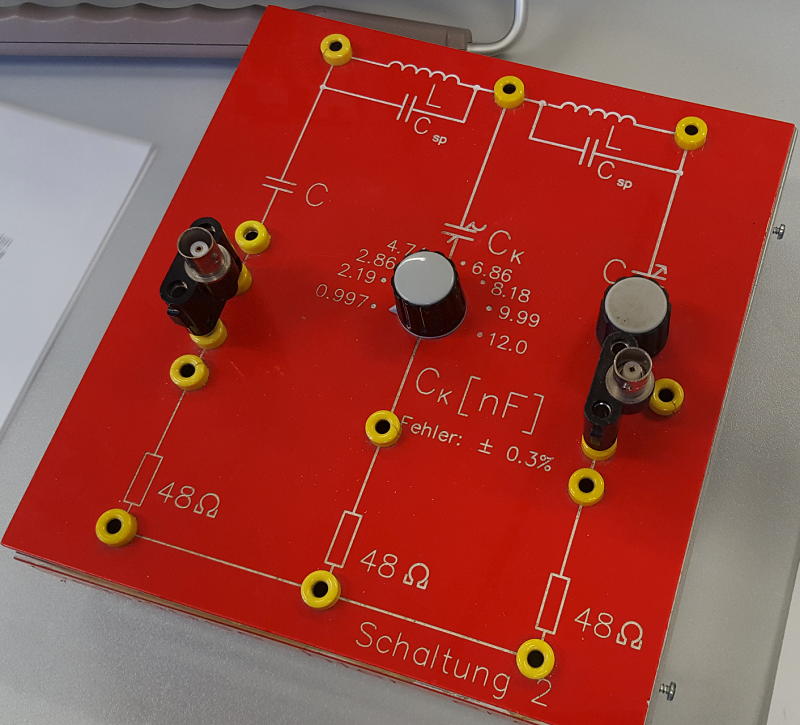
\includegraphics[width=\textwidth/2]{images/foto_01.png}
    \caption{Foto des genutzten Schaltkastens}
    \label{fig:foto_01}
\end{figure}

Gegeben ist der Schaltkasten wie man ihn in \autoref{fig:foto_01} sieht.
Das beide Schwingkreise die gleiche Resonanzfrequenz haben sollen, muss diese für den linken Schaltkreis zunächst ermittelt werden um dann den rechten Schaltkreis daran anzupassen.

\begin{figure}
    \centering
    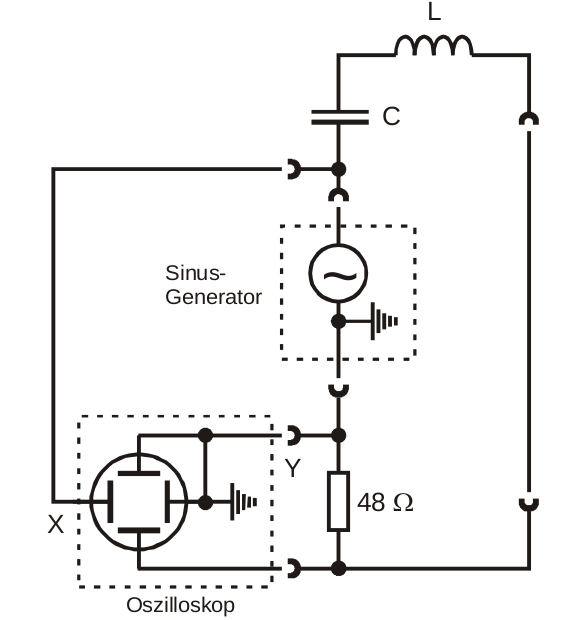
\includegraphics[width=\textwidth/2]{images/schaltung_3.png}
    \caption{Foto des genutzten Schaltkastens}
    \label{fig:schaltung_3}
\end{figure}

Hierzu wird am linken Schwingkreis ein Osziloskop und ein Sinusgenerator wie in \autoref{fig:schaltung_3} angeschlossen. 
Um nun die Resonanzfrequenz zu messen wird am Sinusgenerator die Frequenz solange eingestellt bis die am Oszilloskop abgebildete Lissajous-Figur eine Gerade ist. Nun wird die eingestellte Frequenz als Resonanzfrequenz notiert.
Dann muss die gleiche Schaltung mit gleicher Generatorfrequenz für den rechten Schwingkreis aufgebaut werden.
Der dort eingebaute Kondensator wird nun so eingestellt dass auch hier die Lissajous-Figur eine Gerade ist. Nun sind die Schwingkreise nahezu identisch und die eigentliche Messung kann beginnen.

\subsection{Messung des Schebungs-Schwingungs-Verhältnisses}

\begin{figure}
    \centering
    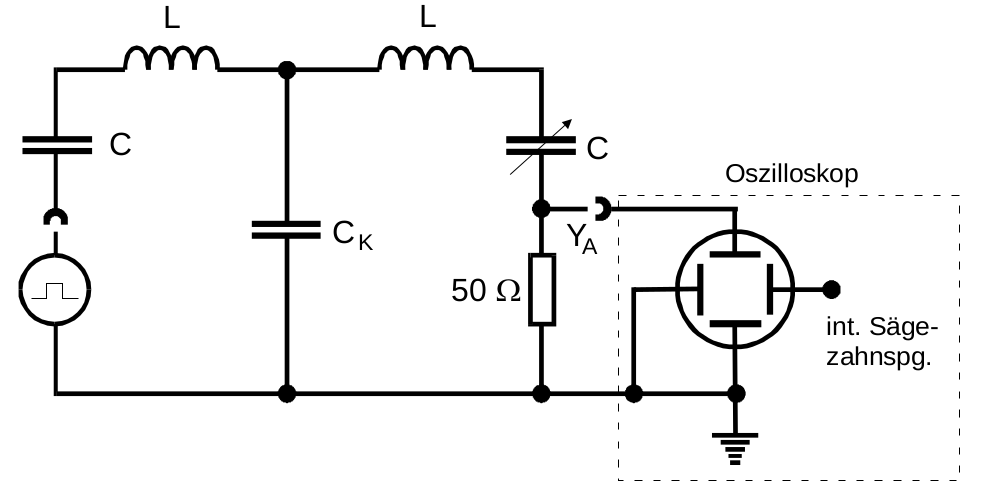
\includegraphics[width=\textwidth/2]{images/schaltung_4.png}
    \caption{Foto des genutzten Schaltkastens}
    \label{fig:schaltung_4}
\end{figure}

Nun wird die Schaltung aus \autoref{fig:schaltung_4} aufgebaut.
Am Generator wird eine Frequenz gesucht, mit der die Schwebung gut am Oszilloskop zu sehen ist. Die Anzahl der Maxima und Extrema innerhalb eines Nulldurchgangs der Schwebung werden abgezählt und notiert. 
Dies wird für verschiedene Kopplungskapazitäten wiederholt.